\newpage
\section{Sprint 2}
\label{sec:sprint2}

Siguiendo la planificación inicial detallada en la sección \ref{sec:planificacion-inicial}, el segundo sprint se enfoca exclusivamente en el desarrollo de la \textbf{aplicación móvil}. El objetivo principal es sentar las bases de la aplicación cliente, creando una estructura de proyecto robusta, implementando los módulos nativos necesarios para funcionalidades clave y desarrollando una primera versión de la interfaz de usuario.

El entregable al final de este sprint será una aplicación de galería básica que pueda solicitar los permisos necesarios, acceder a las fotos y vídeos del dispositivo y mostrarlos en una interfaz de usuario funcional. Aún no se implementarán las funcionalidades de sincronización con el servidor, ya que el foco está en la arquitectura del cliente y su interacción con el sistema operativo móvil.

La velocidad del equipo del sprint anterior se utilizará como referencia, pero al cambiar completamente el contexto de desarrollo (de backend a móvil), se asume una incertidumbre similar a la del primer sprint. La selección de historias se ha realizado buscando un equilibrio entre la creación de la estructura fundamental y la implementación de una primera funcionalidad visible.

\subsection{Historias de usuario}
A continuación, se presentan las historias de usuario y técnicas seleccionadas para este sprint, priorizando la creación del esqueleto de la aplicación móvil y la interacción con el sistema nativo.

Las historias seleccionadas son las siguientes:
\begin{itemize}
    \item HU20: Ver archivos subidos (adaptada a "Ver archivos locales") - 5 PH
    \item HU24: Inicio y cierre de sesión - 5 PH
    \item HU25: Gestión de permisos - 3 PH
    \item HT23: Acceso a la galería - 5 PH
    \item HT24: Comunicación con API - 5 PH
    \item HT29: Pruebas unitarias - 5 PH (parcial)
    \item HT31: Gestión de tokens - 3 PH
    \item HT36: UI responsive - 3 PH
\end{itemize}

La suma total de las historias seleccionadas es de \textbf{34 puntos de historia (PH)}. Aunque el número de puntos es menor que en el sprint anterior, la complejidad de configurar un nuevo entorno de desarrollo móvil y la implementación de módulos nativos justifica una carga de trabajo similar.

Además, se estima una carga extra a la hora de implementar los módulos nativos y la integración con Lynx.js, lo que puede hacer que el esfuerzo real sea comparable al del primer sprint.

La descomposición en tareas de desarrollo de las historias de usuario se pueden encontrar en el apéndice \ref{appendix:sprint2-backlog}.

El total de horas estimadas para las tareas de desarrollo del Sprint 2 es de \textbf{53.5 horas}, cifra que se acerca a la capacidad teórica del sprint (56 horas). La distribución es la siguiente:

\begin{itemize}
    \item HU20 (Ver archivos locales): 13.5 horas
    \item HU24 (Inicio y cierre de sesión): 7.5 horas
    \item HU25 (Gestión de permisos): 4 horas
    \item HT23 (Acceso a la galería): 10.5 horas
    \item HT24 (Comunicación con API): 5.5 horas
    \item HT29 (Pruebas unitarias): 4.5 horas
    \item HT31 (Gestión de tokens): 4 horas
    \item HT36 (UI responsive): 4 horas
\end{itemize}

Se observa que historias técnicas como HT23 (módulo nativo) y HU20 (archivos locales) consumen una parte significativa del tiempo. Esto se debe a la complejidad de implementar módulos nativos y establecer una base sólida para la aplicación móvil. El desarrollo de los módulos nativos se realiza en Kotlin/Java, entorno en el que el equipo no tiene ninguna experiencia previa.

\subsection{Diagrama de Gantt}
A la hora de realizar las tareas se ha priorizado la visualización de una galería funcional en la aplicación. Una vez que se tenga una galería funcional, se implementarán las funcionalidades que tienen que ver con la comunicación con la API. El acceso a la galería (HT23) es una tarea crítica que debe completarse antes de poder implementar la visualización de archivos locales (HU20), es por ello que las tareas relacionadas con la historia técnica van antes que las de la historia de usuario.

\begin{figure}[H]
    \begin{center}
        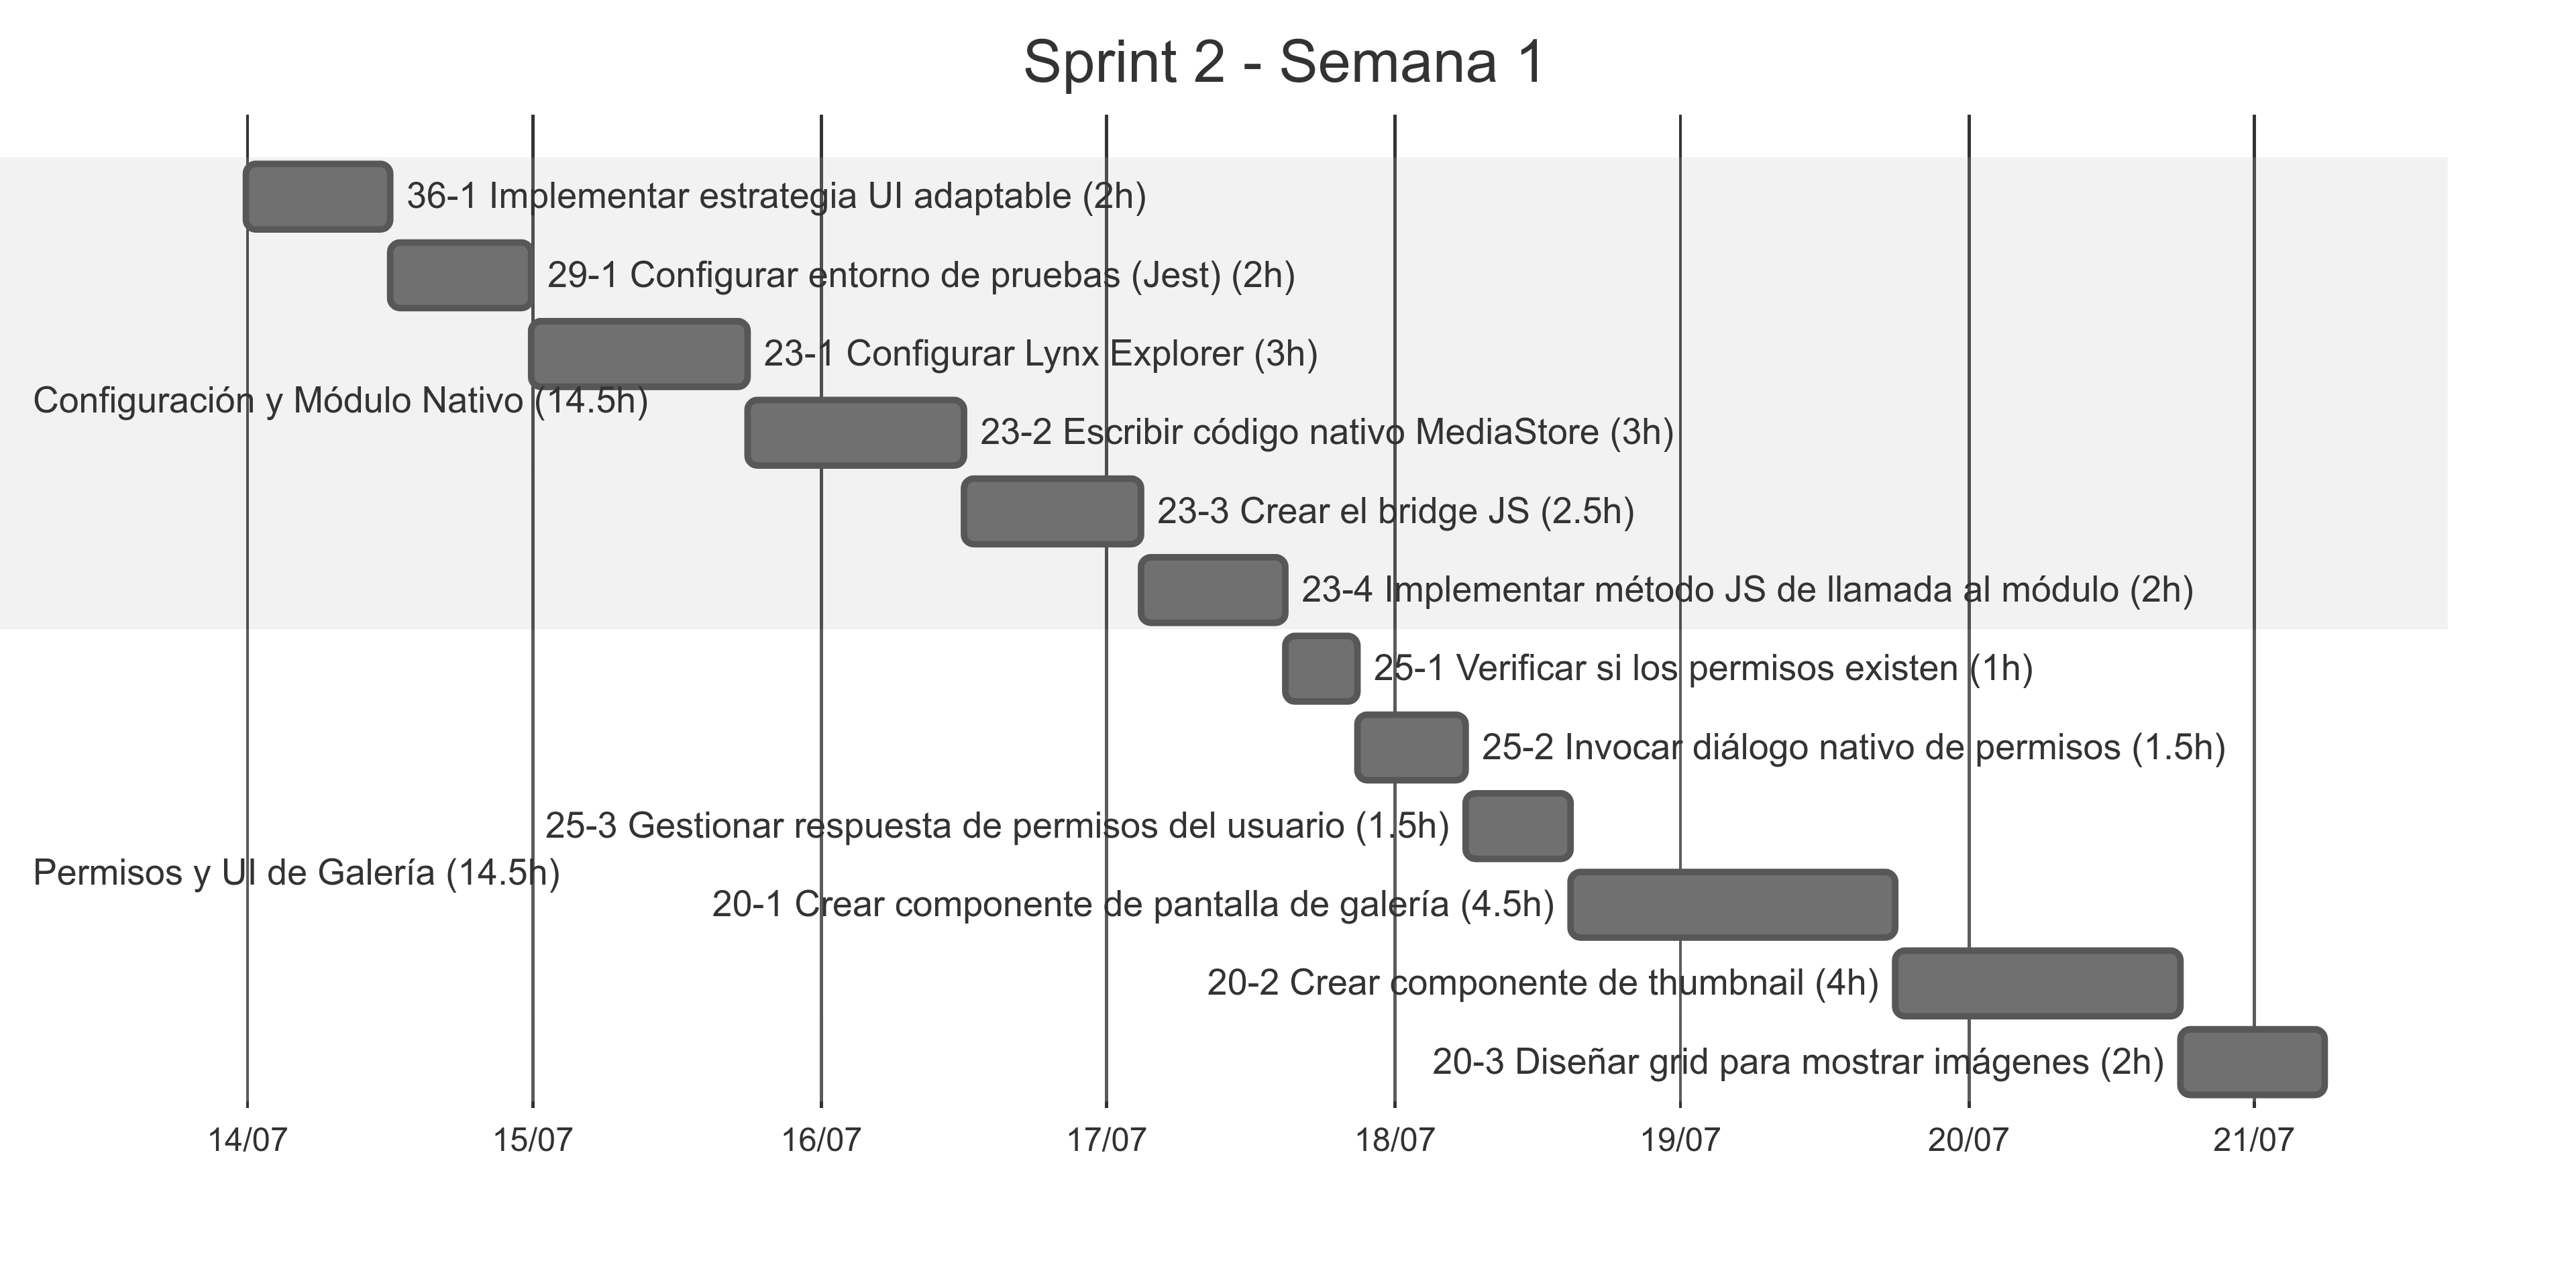
\includegraphics[width=0.8\textwidth]{assets/sprint2/week1-gantt.png}
    \end{center}
    \caption{Diagrama de Gantt de las tareas de la primera semana del sprint 2}\label{fig:gantt-sprint2-week1}
\end{figure}

\begin{figure}[H]
    \begin{center}
        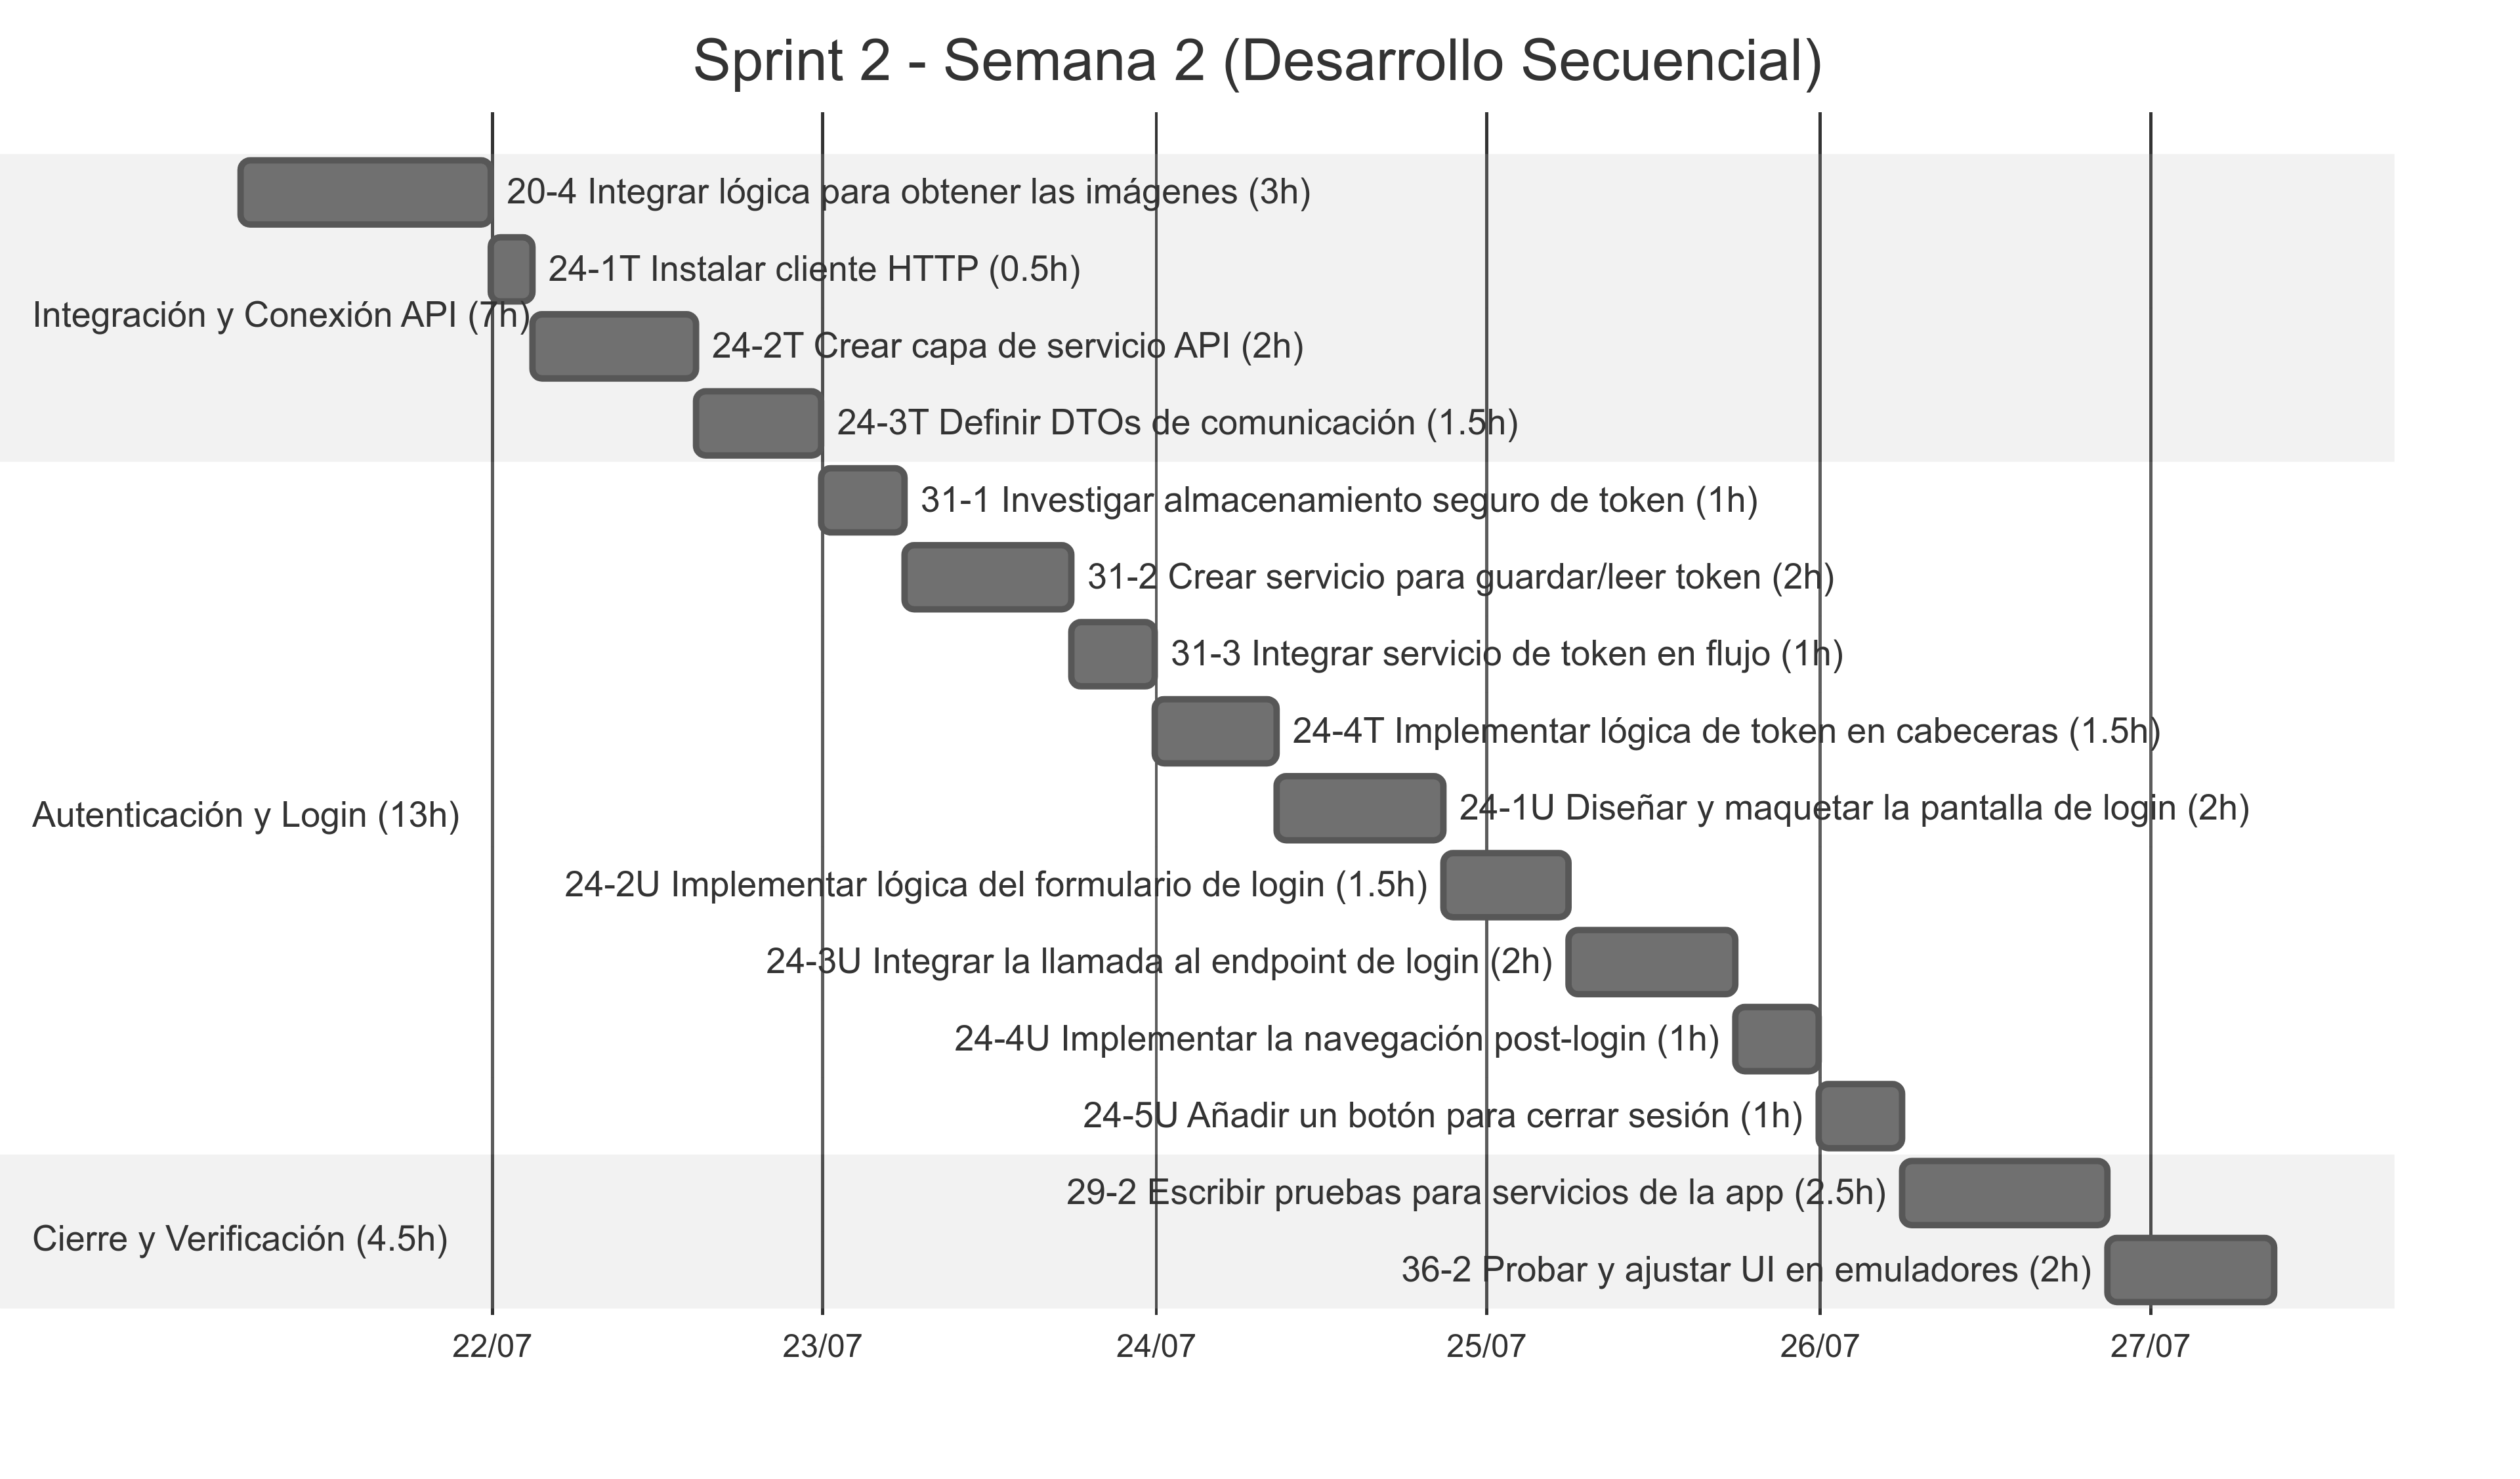
\includegraphics[width=0.8\textwidth]{assets/sprint2/week2-gantt.png}
    \end{center}
    \caption{Diagrama de Gantt de las tareas de la segunda semana del sprint 2}\label{fig:gantt-sprint2-week2}
\end{figure}


\subsection{Diseño detallado e implementación}

\subsubsection{Arquitectura del Cliente Móvil}
Como se definió en la propuesta, la aplicación móvil seguirá los principios de la \textbf{Arquitectura Limpia}. Durante este sprint se materializará esta estructura creando los siguientes directorios y capas lógicas:
\begin{itemize}
    \item \textbf{Presentation}: Contendrá todos los componentes de React (Lynx.js), las pantallas (Login, Galería), y los hooks visuales. Es la capa más externa.
    \item \textbf{Domain}: Albergará las entidades de negocio (ej. `User', `MediaFile') y las definiciones de las interfaces de los repositorios (ej. `AuthRepository', `MediaRepository'). Esta capa no tendrá dependencias externas.
    \item \textbf{Application}: Contendrá los casos de uso (ej. `loginUser', `getLocalMediaFiles'). Orquestará el flujo de datos entre la `Presentation' y el `Domain', usando las interfaces de los repositorios.
    \item \textbf{Infrastructure}: Aquí residirán las implementaciones concretas de las interfaces del dominio. Se creará un `ApiAuthRepository' que use el cliente HTTP (HT24) y un `NativeMediaRepository' que use el módulo nativo implementado (HT23) para acceder a los ficheros del dispositivo.
\end{itemize}

\subsubsection{Implementación de Módulos Nativos en Lynx.js}
El reto técnico principal de este sprint es la creación de un módulo nativo para acceder a la galería (HT23). El proceso seguirá la documentación oficial de Lynx.js, que implica:
\begin{enumerate}
    \item Clonar y configurar el proyecto de `Lynx Explorer' para Android.
    \item En Android Studio, crear una nueva clase Java/Kotlin que herede de `LynxModule'.
    \item Dentro de esta clase, usar las APIs nativas de Android (`ContentResolver' y `MediaStore') para consultar las imágenes y vídeos del dispositivo. Este método también gestionará la solicitud de permisos (`READ\_MEDIA\_IMAGES').
    \item Exponer los métodos necesarios a JavaScript usando la anotación `@LynxMethod'.
    \item Registrar el módulo en la aplicación `Lynx Explorer'.
    \item Compilar una nueva versión del `Lynx Explorer.apk' que incluya nuestro módulo.
    \item Desde el código JavaScript de nuestra aplicación, podremos importar y llamar a este módulo para obtener los datos de la galería.
\end{enumerate}
Este proceso asegura un rendimiento nativo para una tarea intensiva como es el acceso a ficheros multimedia.

\subsubsection{Implementación de botón de retroceso en Android}
Aunque puede ser algo que se da por echo en un framework móvil, es importante destacar que Lynx.js no implementa por defecto el botón de retroceso.
El comportamiento por defecto es el de salir de la aplicación al pulsar el botón de retroceso, lo cual no es deseable en una aplicación que tiene múltiples pantallas y donde se espera que el usuario pueda navegar hacia atrás sin salir de la app.

Para la navegación es ha hecho uso de la librería `react-router`, que permite gestionar las rutas y la navegación entre pantallas de forma sencilla.
Sin embargo, el botón de retroceso del dispositivo no está gestionado automáticamente por esta librería, lo que puede llevar a una experiencia de usuario inconsistente.

Para solucionar este problema, se ha implementado un componente que captura un evento lanzado por la parte nativa de Android cuando se pulsa el botón de retroceso.
Al recibir el evento, el componente navega a la pantalla anterior si existe, o cierra la aplicación si se está en la pantalla principal.

La implementación en Lynx.js sería de la siguiente manera:
\begin{lstlisting}[language=typescript, caption={Implementación del botón de retroceso en Lynx.js}]
export function BackButtonHandler() {
  const nav = useNavigate();
  const handleBackButton = useCallback(() => {
    nav(-1);
  }, [nav]);
  useLynxGlobalEventListener('backButtonPressed', handleBackButton);
  return null;
}
\end{lstlisting}
Este componente se incluye en la parte superior de la jerarquía de componentes, asegurando que captura el evento de retroceso en cualquier pantalla de la aplicación.

La implementación del evento `backButtonPressed` en la parte nativa de Android queda de la siguiente manera:
\begin{lstlisting}[language=Java, caption={Implementación del evento de botón de retroceso en Android}]
backButtonCallback = new OnBackPressedCallback(true) {
    @Override
    public void handleOnBackPressed() {
        if (mLynxView != null && mLynxView.getContext() instanceof LynxContext) {
            ((LynxContext) mLynxView.getContext()).sendGlobalEvent("backButtonPressed", null);
        }
    }
};
getOnBackPressedDispatcher().addCallback(this, backButtonCallback);
\end{lstlisting}
El registro del componente se realiza en la actividad principal de la aplicación, asegurando que el evento se envía a la capa de JavaScript cuando el usuario pulsa el botón de retroceso.

\subsubsection{Implementación de componente input}

Aunque Lynx.js proporciona componentes básicos como `view', `text' y `image', no incluye un componente de entrada de texto (`input') por defecto.
Para implementar un campo de entrada de texto, se ha creado un componente personalizado que encapsula la funcionalidad básica de un campo de texto.

Para la implementación del componente, se ha tenido que utilizar el componente nativo `AppCompatEditText' de Android, que permite al usuario introducir texto.
Gracias a la flexibilidad de Lynx.js (\cite{lynx-documentation}, \href{https://lynxjs.org/guide/custom-native-component.html#platform=android}{Implementando un componente nativo}), se ha podido crear un componente que se comporta como un campo de entrada de texto estándar en React Native teniendo el control total de la implementación.
